



\subsection{CoqIDE version 8.10.2}
	


\begin{minipage}{\linewidth}
\center{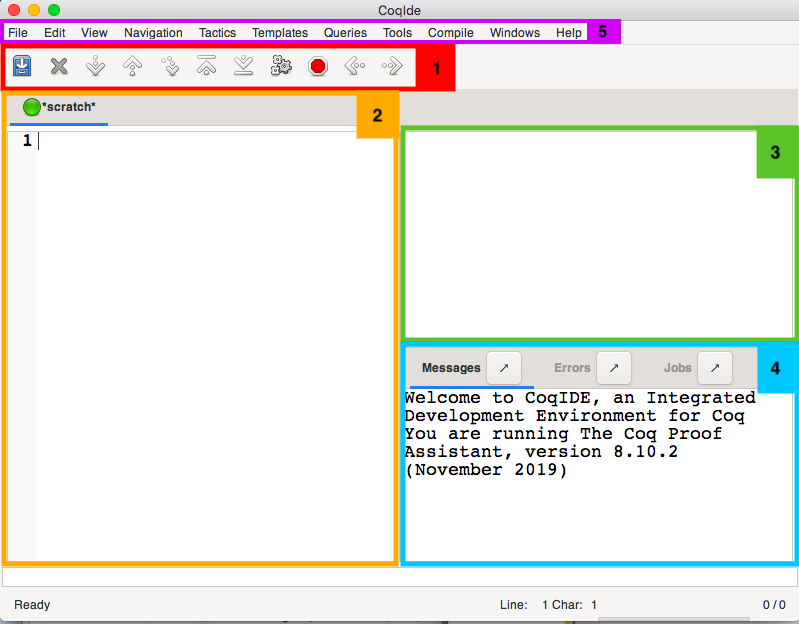
\includegraphics[width=\textwidth]
        {CoqScreenshots/CoqIDEv8_10_2_color.png}}
        \label{fig:IDEcolor} 
        \captionof{figure}{CoqIDE v8.10.2  
        (1) Toolbar. (2) Script Buffer. (3) Goal Window. (4) Message Window. }
\end{minipage}

\subsubsection{Toolbar for CoqIDE v8.10.2}
\hspace{-0.75cm}
\begin{tabular}{ C L }
\centered{
\includegraphics[width=\iconsize]
        {CoqScreenshots/save_10.png}}
        & \centeredl{Save current buffer. 
        If it hasn't been previously saved, functions as save as; use the extension .v to save as a Coq file.
        } \\ \\
\centered{
\includegraphics[width=\iconsize]
        {CoqScreenshots/close_10.png}}
	& \centeredl{Close current buffer. 
	Gives a warning if the file has unsaved changes.
	} \\ \\
\centered{
\includegraphics[width=\iconsize]
        {CoqScreenshots/step_forward_10.png}}
	& \centeredl{Forward one command.
	Steps forward to evaluate the next command in the current file.
	} \\ \\
\centered{
\includegraphics[width=\iconsize]
        {CoqScreenshots/step_backward_10.png}}
	& \centeredl{Backward one command.
	Steps backward one command in the file, returns the state to where it was before evaluating that command. 
	} \\ \\ 
\centered{
\includegraphics[width=\iconsize]
        {CoqScreenshots/go_to_cursor_10.png}}
	& \centeredl{Go to cursor.
	Evaluate all commands in file up to where the cursor currently is.
	} \\ \\ 
\centered{
\includegraphics[width=\iconsize]
        {CoqScreenshots/go_to_top_10.png}}
	& \centeredl{Restart Coq.
	Returns to the top of the file, where no commands have been evaluated.
	} \\ \\ 
\centered{
\includegraphics[width=\iconsize]
        {CoqScreenshots/go_to_bottom_10.png}}
	& \centeredl{Go to end.
	Evaluate to the bottom of the file. 
	Does not work as well with load commands and require import commands.
	} \\ \\
\centered{
\includegraphics[width=\iconsize]
        {CoqScreenshots/check_10.png}}
	& \centeredl{Fully check the document.
	Submits proof terms to the Coq kernel for type checking.
	} \\ \\
\centered{
\includegraphics[width=\iconsize]
        {CoqScreenshots/stop_10.png}}
	& \centeredl{Interrupt computations.
	Stops computation at whatever point was reached before pressing the button.
	} \\ \\
\centered{
\includegraphics[width=\iconsize]
        {CoqScreenshots/next_occurrence_10.png}}
	& \centeredl{Next Occurrence.
	Goes to the next occurrence of whatever the cursor is currently by. 
	Works well for longer words.
	} \\ \\
\centered{
\includegraphics[width=\iconsize]
        {CoqScreenshots/previous_occurrence_10.png}}
	& \centeredl{Previous Occurrence.
	Goes to the previous occurrence of whatever the cursor is currently by.
	Works well for longer words.
	}
\end{tabular}










\subsection{CoqIDE version 8.7.2}
	


\begin{minipage}{\linewidth}
\center{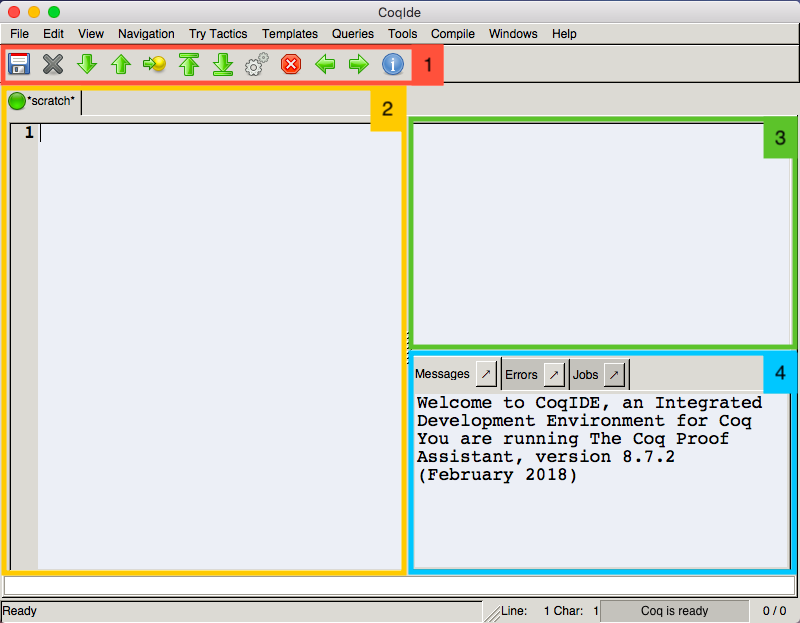
\includegraphics[width=\textwidth]
        {CoqScreenshots/CoqIDE_color.png}}
        \label{fig:IDEcolor} 
        \captionof{figure}{CoqIDE v8.7.2  
        (1) Toolbar. (2) Script Buffer. (3) Goal Window. (4) Message Window. }
\end{minipage}


\subsubsection{Toolbar for CoqIDE v8.7.2}
\hspace{-0.75cm}
\begin{tabular}{ C L }
\centered{
\includegraphics[width=\iconsize]
        {CoqScreenshots/save.png}}
        & \centeredl{Save current buffer. 
        If it hasn't been previously saved, functions as save as; use the extension .v to save as a Coq file.
        } \\ \\
\centered{
\includegraphics[width=\iconsize]
        {CoqScreenshots/close.png}}
	& \centeredl{Close current buffer. 
	Gives a warning if the file has unsaved changes.
	} \\ \\
\centered{
\includegraphics[width=\iconsize]
        {CoqScreenshots/step_forward.png}}
	& \centeredl{Forward one command.
	Steps forward to evaluate the next command in the current file.
	} \\ \\
\centered{
\includegraphics[width=\iconsize]
        {CoqScreenshots/step_backward.png}}
	& \centeredl{Backward one command.
	Steps backward one command in the file, returns the state to where it was before evaluating that command. 
	} \\ \\ 
\centered{
\includegraphics[width=\iconsize]
        {CoqScreenshots/go_to_cursor.png}}
	& \centeredl{Go to cursor.
	Evaluate all commands in file up to where the cursor currently is.
	} \\ \\ 
\centered{
\includegraphics[width=\iconsize]
        {CoqScreenshots/go_to_top.png}}
	& \centeredl{Restart Coq.
	Returns to the top of the file, where no commands have been evaluated.
	} \\ \\ 
\centered{
\includegraphics[width=\iconsize]
        {CoqScreenshots/go_to_bottom.png}}
	& \centeredl{Go to end.
	Evaluate to the bottom of the file. 
	Does not work as well with load commands and require import commands.
	} \\ \\
\centered{
\includegraphics[width=\iconsize]
        {CoqScreenshots/check.png}}
	& \centeredl{Fully check the document.
	Submits proof terms to the Coq kernel for type checking.
	} \\ \\
\centered{
\includegraphics[width=\iconsize]
        {CoqScreenshots/stop.png}}
	& \centeredl{Interrupt computations.
	Stops computation at whatever point was reached before pressing the button.
	} \\ \\
\centered{
\includegraphics[width=\iconsize]
        {CoqScreenshots/next_occurrence.png}}
	& \centeredl{Next Occurrence.
	Goes to the next occurrence of whatever the cursor is currently by. 
	Works well for longer words.
	} \\ \\
\centered{
\includegraphics[width=\iconsize]
        {CoqScreenshots/previous_occurrence.png}}
	& \centeredl{Previous Occurrence.
	Goes to the previous occurrence of whatever the cursor is currently by.
	Works well for longer words.
	} \\ \\
\centered{
\includegraphics[width=\iconsize]
        {CoqScreenshots/proof_wizard.png}}
	& \centeredl{Proof Wizard. 
	Tries to apply a given set of tactics in order. 
	The tactics to be attempted can be customized by going to: 
	Edit tab $\to$ Preferences, then select Tactics Wizard in the leftmost pane of the Customizations window.} 
\end{tabular}












\subsection{Script Buffer}
Here you can type out new definitions and proofs in a new buffer, or open a buffer from a saved file by going to the File tab $\to$ Open, then choosing the file. 
You can edit and save new and existing buffers here. 
\begin{code} 
	This block represents a script buffer in this tutorial. 
\end{code}



\subsection{Goal Window}
Goals to be proven will be displayed here. 
This window will be empty unless you're in a proof environment; inside the proof environment, it will display what you goal are currently proving, what goals are left to be proved, or that there are no more subgoals and your proof is complete.
\begin{goal} 
	This block represents the goal window in this tutorial. 
\end{goal}



\subsection{Message Window}
Any messages resulting from an executed command will be displayed here. 
Results from queries are also printed out here. 
Clicking the arrow in the corner of the Messages, Errors, or Jobs tab here will create a separate window for that tab. 
When the separate window is closed, it will return to the main Coq IDE window. 
\begin{msg} 
	This block represents the message window in this tutorial. 
\end{msg}















